% last updated in April 2002 by Antje Endemann
% Based on CVPR 07 and LNCS, with modifications by DAF, AZ and elle, 2008 and AA, 2010, and CC, 2011; TT, 2014

\documentclass[runningheads]{llncs}
\usepackage{graphicx}
\usepackage{amsmath,amssymb} % define this before the line numbering.
\usepackage{ruler}
\usepackage{color}
\usepackage{array}
\usepackage{float}
\usepackage{subfig,caption}
\usepackage{lipsum}
\usepackage{dcolumn}



%\usepackage{subcaption}
\usepackage{comment}
\renewcommand{\arraystretch}{1.1}
\usepackage[width=122mm,left=12mm,paperwidth=146mm,height=193mm,top=12mm,paperheight=217mm]{geometry}
\begin{document}
% \renewcommand\thelinenumber{\color[rgb]{0.2,0.5,0.8}\normalfont\sffamily\scriptsize\arabic{linenumber}\color[rgb]{0,0,0}}
% \renewcommand\makeLineNumber {\hss\thelinenumber\ \hspace{6mm} \rlap{\hskip\textwidth\ \hspace{6.5mm}\thelinenumber}}
% \linenumbers
\pagestyle{headings}
\mainmatter
\def\ECCV14SubNumber{1355}  % Insert your submission number here

\title{Analyzing The Performance of Multilayer Neural Networks for Object Recognition: Supplementary Material} % Replace with your title

\titlerunning{ECCV-14 submission ID \ECCV14SubNumber}

\authorrunning{ECCV-14 submission ID \ECCV14SubNumber}

\author{Anonymous ECCV submission}
\institute{Paper ID \ECCV14SubNumber}


\maketitle


\section{On Using Entropy For Measuring Change in Selectivity}
\subsection{Motivation}
In answer to question -``What happens when a discriminatively pretrained network is fine-tuned" (sec 3 of the main paper) we used entropy of filters and entropy of layers as a measure of how selective each layer is. The choice of entropy is motivated by: Entropy naturally measures how selective a particular feature is across different classes and not just individual classes. Consequently, entropy has been extensively used in a lot of computer vision applications based on decision trees such as \cite{AmitGeman} \cite{Breiman}.

\subsection{Method of Entropy Computation}
We presented a natural way of computing entropy of each unit of every layer in sec 2.3 of the paper. We call this Label-Entropy. However, one might also compute entropy of units in other ways. We considered two more methods as described below.

We define the entropy of a filter with respect to a given set of image-label pairs in the following way. Each image, when passed through the convolutional neural network produces a $p \times p$ heatmap of filter responses. (eg p = 6, for a layer 5 filter). Further assume that there are $C$ classes.
\subsubsection{Label Entropy}
\label{sub:def-label-ent}
We vectorize the heatmap into a vector of scores of length $p^2$ and with each element of this vector we associate the class label of the image. Thus, for each image we have a score vector and a label vector of length $p^2$ each. Next, we concatenate score vectors and label vectors from N images into a giant score vector and a giant label vector  of size $Np^2$ each. Now for every score threshold $(t)$ we consider all the labels which have an associated score $\geq t$. We construct a normalized histogram of label counts from this set of labels. The entropy of this histogram is the entropy of the filter at this threshold. As this threshold changes, entropy traces out a curve which we call as the entropy curve.  

\subsubsection{Weighted Label Entropy}
\label{sub:def-weighted-label-ent}
When computing the label histogram as described above, instead of the label count we use the sum of the scores associated with the labels to construct the histogram. (Note: Since we are using outputs from relu or rectified linear units, all scores are $\geq 0$.)

\subsubsection{Spatial-Max (spMax) Label Entropy}
\label{sub:def-spmax-label-ent}
From the heatmap, we chose the element which has the maximum value and associate with it the label of the image class. Thus, for each image we have a score vector and a label vector of length $1$ each. Next, we concatenate score vectors and label vectors from N images into a  score vector and a  label vector  of size $N$ each. Now for every score threshold $(t)$ we consider all the labels which have an associated score $\geq t$. Next, we compute the entropy as in the case of Label-Entropy.

\subsection{Mean Cumulative Area Under Entropy Curve (MCAuE Index)}
In order to compute entropy of the layer, we introduced the notions of Area Under the Entropy Curve and Mean Cumulative Area Under Entropy Curve (MCAuE) analogous to the notion of computing area under Mean Average-Precision (\cite{Pascal}) in sec 3 and fig 2 of the main paper. However due to space constraints we could only provide a brief definition of MCAuE index. A detailed definition is as following:

For each filter in the layer we first calculate the area under entropy (AuE) curve. Next, filters are sorted according to their AuE. Then, we calculate the Cumulative Area under Entropy (CAuE) by computing the cumulative sum of sorted list of AuE of all filters of this layer. Finally, to normalize for the number of filters we divide the $i^{th}$ entry of the CAuE list by $i$. This results into a number which we call as the Mean Cumulative Area Under the Entropy Curve (MCAuE). In order to compare different layers, we compare MCAuE at 30 threshold points. The  $k^{th}$ threshold point for layer l corresponds to MCAuE of top $N_l(k/30)$ filters, where $N_l$ is number of filters in layer $l$.


\setlength{\tabcolsep}{1pt}
\begin{table}
\begin{center}
\caption{This table lists percentage decrease in MCAuE as a result of finetuning when only 0.1, 0.25, 0.50 and 1.00 fraction of all the filters were used for computing MCAuE. A lower MCAuE indicates that filters in a layer are more selective/class specific. The 0.1 fraction includes the top 10\% most selective filters, 0.25 is top 25\% of most selective filters. Consequently, comparing MCAuE at different fraction of filters gives a better sense of how selective the ``most" selective filters have become to how selective all the filters have become.
A negative value in the tabel below indicates increase in entropy. Note that for all the metrics maximum decrease in entropy takes place while moving from layer 5 to layer 7. Also, note that for relu-6 and relu-7 the values in Label-Entropy and spMax-Label-Entropy are same as relu-6 and 7 have spatial maps of size 1.}
\label{table:fine-change}
\scalebox{0.85}{
\newcolumntype{d}[2]{D{.}{\cdot}{#1} }
\begin{tabular}{|c|p{1cm} p{1cm} p{1cm} p{1cm}| p{1cm} p{1cm} p{1cm} p{1cm}|p{1cm} p{1cm} p{1cm} p{1cm}|}
\hline
Layer & \multicolumn{4}{c|}{Label-Entropy} & \multicolumn{4}{c|}{Weighted-Label-Entropy} & \multicolumn{4}{c|}{spMax-Label-Entropy} \\
\hline
& 0.1 & 0.25 & 0.5 & 1.0 & 0.1 & 0.25 & 0.5 & 1 & 0.1 & 0.25 & 0.5 & 1.0 \\
\hline
pool-1 & $-0.02$  & $-0.14 $  & $-0.19$  & $-0.19$  & $0.06$  & $-0.13$  & $-0.16$  & $-0.16$  & $0.19$  & $0.10$  & $0.07$  & $0.04$   \\
pool-2 & $-0.71$  & $-0.31$   & $-0.14$  & $0.01$  & $0.41$  & $0.53$  & $0.58$  & $0.57$  & $-0.39$  & $-0.03$  & $0.11$  & $0.23$  \\ 
relu-3 & $-1.14$  & $-0.86$   & $-0.67$  & $-0.44$ & $1.11$  & $0.66$  & $0.52$  & $0.32$ & $0.14$  & $0.20$  & $0.32$  & $0.33$   \\
relu-4 & $-0.54$  & $-0.31$  & $-0.19$  & $-0.05$ & $-0.10$  & $0.55$  & $0.64$  & $0.57$  & $0.93$  & $0.97$  & $0.80$  & $0.65$ \\
pool-5 & $0.97$  & $0.55$  & $0.43$  & $0.36$ & $5.84$  & $3.53$  & $2.66$  & $1.85$  & $4.87$  & $3.05$  & $2.31$  & $1.62$   \\
relu-6 & $6.52$  & $5.06$  & $3.92$  & $2.64$  & $9.59$  & $7.55$  & $6.08$  & $4.27$ & $6.52$  & $5.06$  & $3.92$  & $2.64$   \\
relu-7 & $5.17$  & $2.66$  & $1.33$  & $0.44$  & $20.58$  & $14.75$  & $11.12$  & $7.78$  & $5.17$  & $2.66$  & $1.33$  & $0.44$  \\
\hline
\end{tabular}}
\end{center}
\end{table}
\setlength{\tabcolsep}{1.4pt}

\begin{figure}
\centering
\subfloat{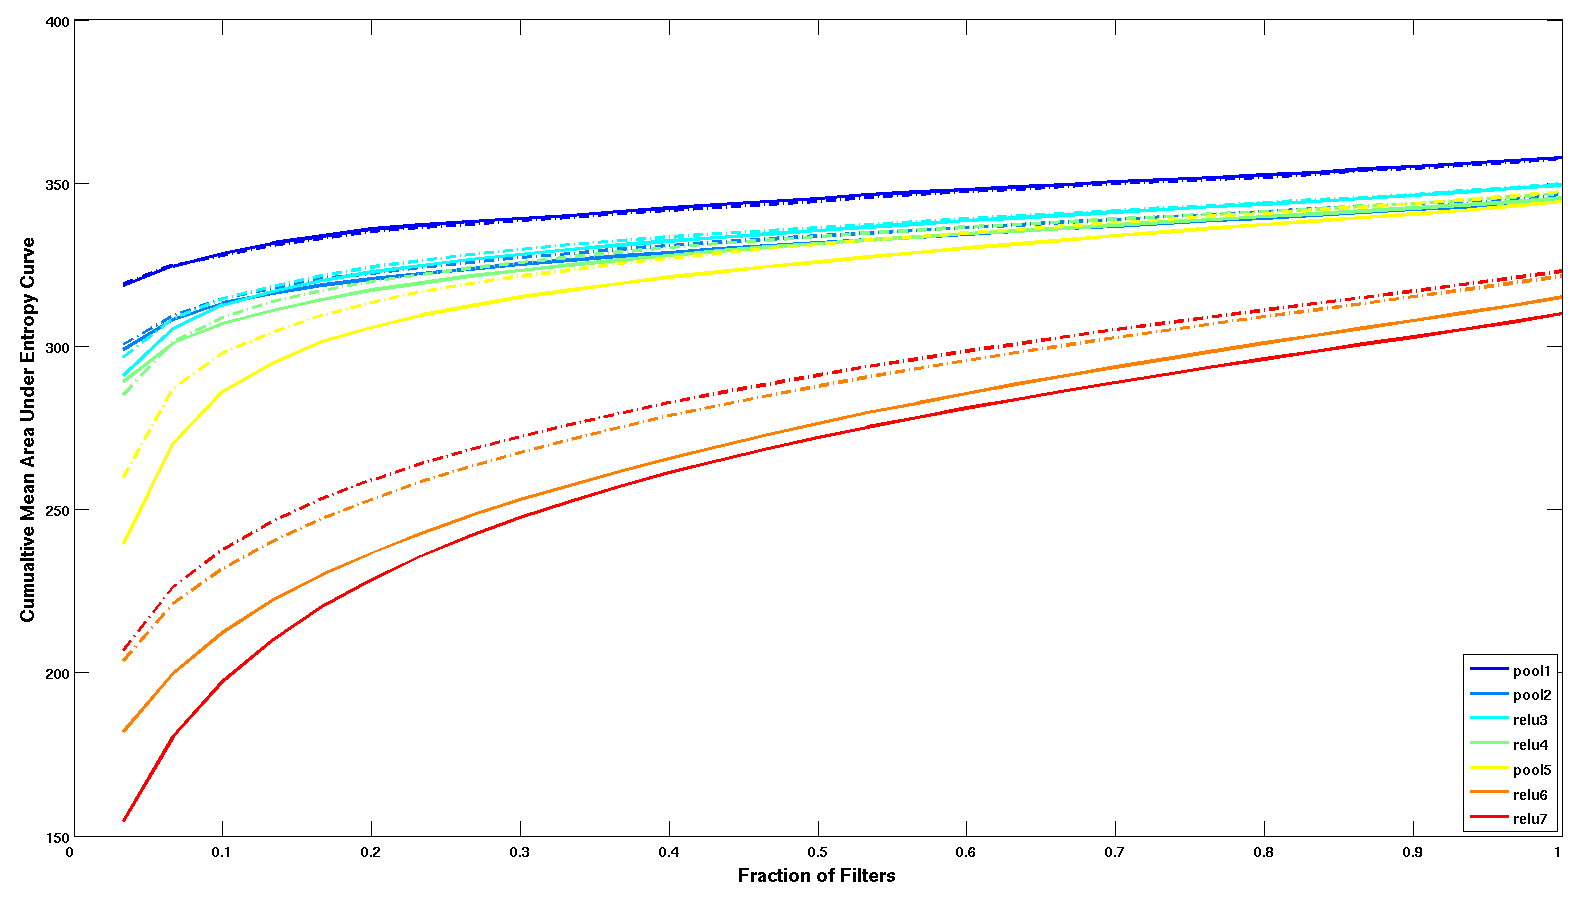
\includegraphics[scale=0.15]{images/weighted_layer_entropy.png}} \\
\subfloat{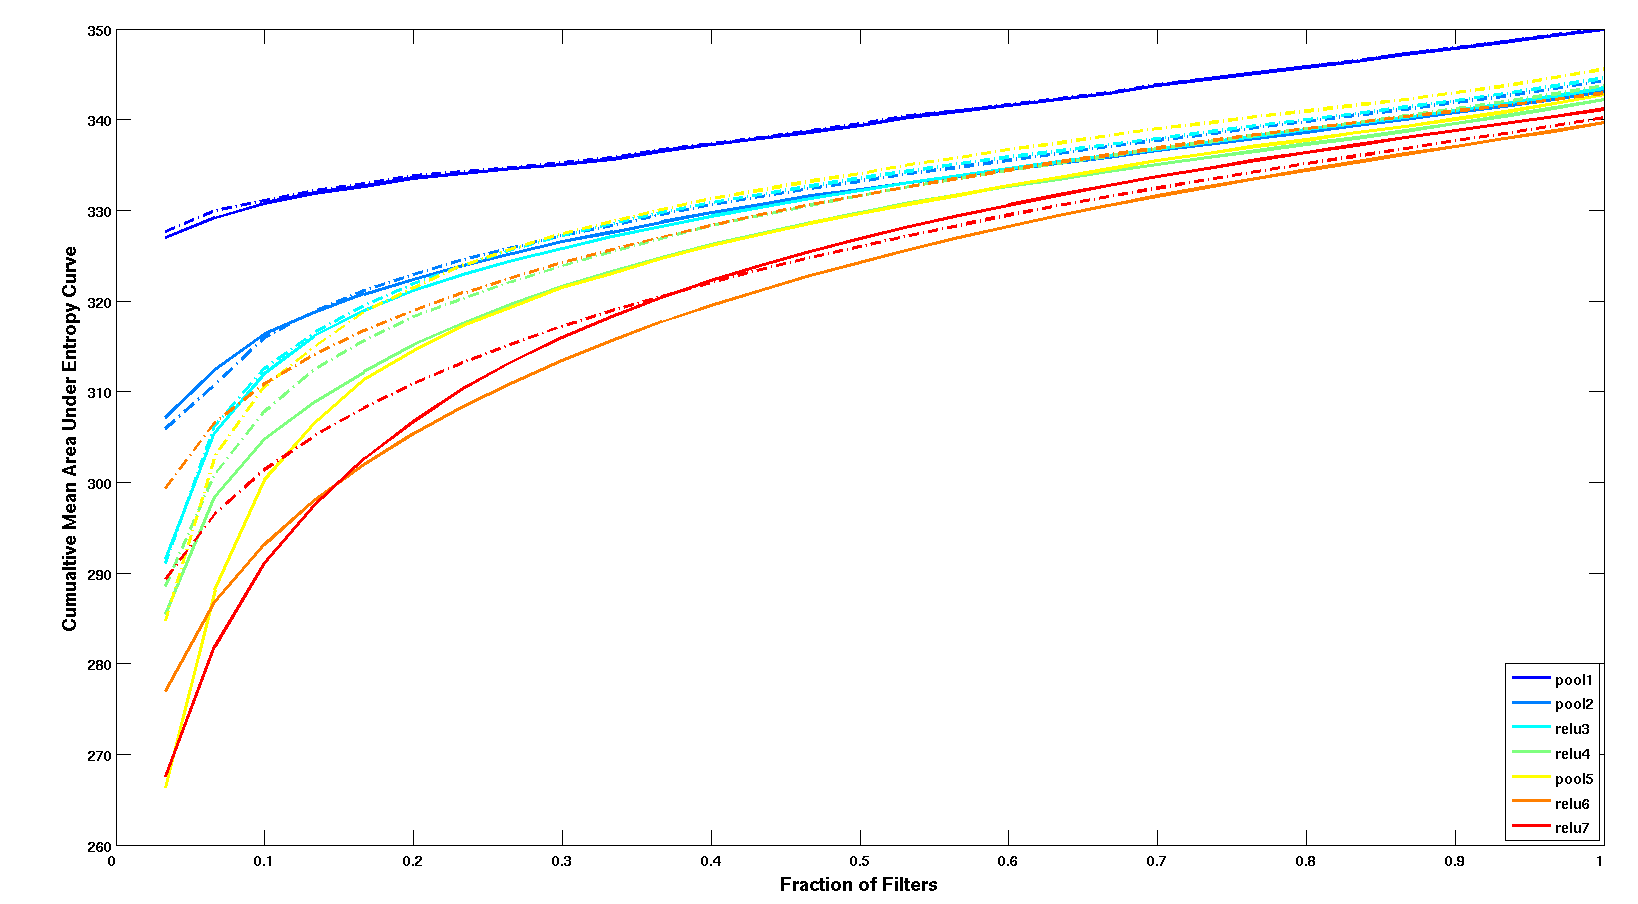
\includegraphics[scale=0.15]{images/spmax_layer_entropy.png}}
\caption{Mean Cumulative AuE plotted as fraction of filters for all layers of the Conv-Net. Dash-Dot Line: Alex-Net, Solid Line: Fine-Tuned Network. The top plot shows entropy calculated using Weighted-Label-Entropy Method, whereas the bottom plot entropy calculated using spMax-Label-Entropy Method. (see sec \ref{sub:def-label-ent} for method definitions.)}
\label{fig:fine-entropy}
\end{figure}

\subsection{Discussion}
The change in MCAuE for different layers as measured using alternative definitions of entropy can be seen in fig \ref{fig:fine-entropy} (Please see sec 3 of the main paper for more details on the procedure). A quantitative measure of change in entropy after finetuning is provided in table \ref{table:fine-change}. The percentage change in MCAuE is calculated as:
\begin{eqnarray}
\text{Percent Decrease} = 100 \times \frac{MCAuE_{untuned} - MCAuE_{fine}}{MCAuE_{untuned}}
\end{eqnarray}
where, $MCAuE_{fine}$ is for fine-tuned network and $MCAuE_{untuned}$ is for network trained on imagenet only.

Although, the most natural way to compute entropy is Label-Entropy as used by \cite{Breiman}, \cite{AmitGeman}, the alternative metrics also support the claim that most of the changes due to fine-tuning happen while moving from layers 5 to 7. At the same time, it is noteworthy, that for label-entropy pool-5 undergoes negligible change in entropy, whereas changes in pool-5 as measured by Weighted-Label Entropy and spMax-Label-Entropy are comparable to changes in relu-6 and relu-7.

\section{On Grand-Mother Cells}
\begin{figure}[t!]
\centering
\subfloat{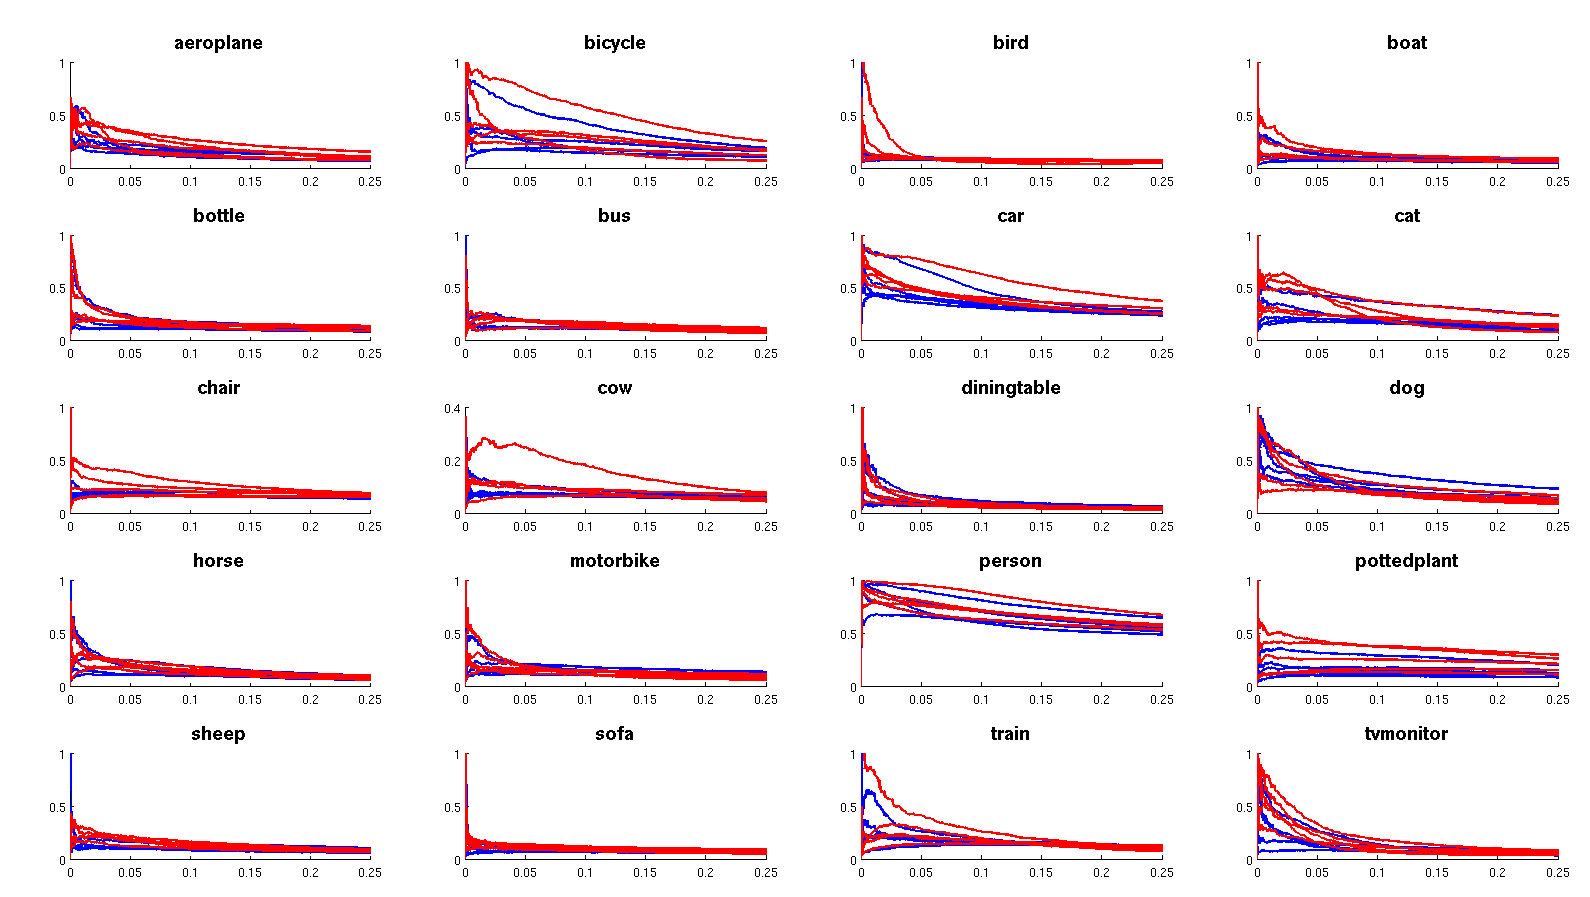
\includegraphics[scale=0.20]{images/gtbbox_pascal_prerec_pool5units.png}}
\caption{Precision-Recall Curves for 20 PASCAL Classes calculated using pool-5 filter responses on ground truth bounding boxes. Red-Curves: Fine Tuned Network, Blue-Curves: Alex-Net. The figure only displays 5 best filters for each class based on AP  upto a recall threshold of 0.25. For most classes, precision drops significantly even at modest recall values.}
\label{fig:ap}
\end{figure}

Originally, Grand-Mother Cells were described as ``hypothetical" neurons in the brain which only respond to very specific visual stimulus \cite{Barlow} \cite{Grandmother}. Mathematically, these can be expressed as high precision units and we presented this analysis in sec 5.1 of our main paper. Although, presence/absence of Grand-Mother is a scientifically  interesting question to pursue - for recognition, only filters with high precision are not sufficient. We also require high recall. Consequently we also analyzed if there are pool-5 units which have high AP. Figure \ref{fig:ap} plots precision-recall curves of 5 filters with highest AP for each of the PASCAL classes.

From this figure, it is clear that even at modest recalls, for most of the classes precision degrades quite fast. Its only for a few classes such as Person, Bicycle, Cars that we have filters which have relatively high AP values. These results further cement the conjecture that indeed the mid-level representations in these networks are distributed.

\section{Epoch Numbers}
The Imagenet Training(Alex-Net) was performed using 310000 iterations, which corresponds to 66 epochs. (1 epoch is one pass over the entire training set.) For fine-tuning, we used a scheme closely following \cite{Rcnn} which samples positives with a higher probability as compared to the negatives and hence reporting epoch numbers is not insightful. Please look into \cite{Rcnn} for more details.

\bibliographystyle{splncs}
\bibliography{egbib}
\end{document}
